\chapter{拉格朗日量、場與局域粒子過程}

玻色子場、費米子場和電磁場都遵循波動方程。這些方程涉及場本身，以及場對空間和時間的導數。雖然可以為每個場分別列出運動方程，但拉格朗日量能將整個系統濃縮為一個表示式。將尤拉--拉格朗日法則應用於這個表示式，就能一次得到所有場的方程。

這種構造與作用量取駐值密切相關。此處的直接目標更為具體：確認場的拉格朗日量依賴哪些量，用它推導幾個經典方程，再以量子力學的觀點重新詮釋相同的場表示式。在量子理論中，拉格朗日量支配粒子的運動與交互作用，最終也決定碰撞的振幅與截面。

\section{場方程的簡潔表述}

對於單一標量場，拉格朗日密度取決於場及其一階導數，
\begin{equation}
\mathcal L
=
\mathcal L\!\left(\phi,\partial_t\phi,\partial_x\phi,\ldots\right)
=
\mathcal L\!\left(\phi,\partial_\mu\phi\right).
\end{equation}
計算時，明確列出時間導數與空間導數往往更方便；記號\(\partial_\mu\phi\)則以相對論形式概括同一組導數。

\begin{figure}[htbp]
\centering
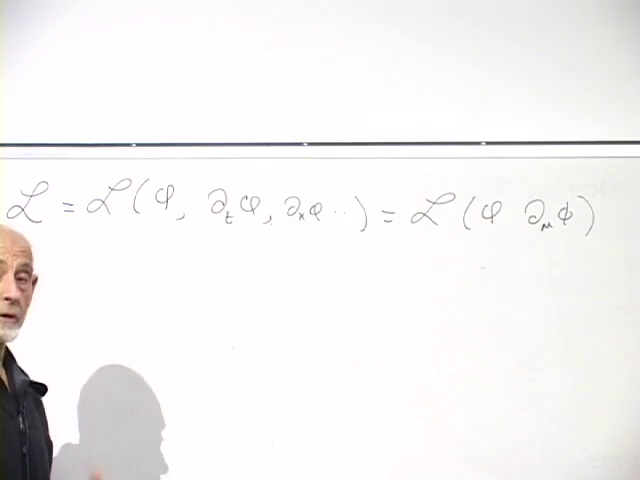
\includegraphics[width=0.82\textwidth]{lecture_09_figure_03.png}
\caption{標量場的拉格朗日量對場及其時空導數的依賴關係。}
\lectureframe{00:03:56}
\end{figure}

場的尤拉--拉格朗日方程為
\begin{equation}
\frac{\partial}{\partial t}
\frac{\partial\mathcal L}{\partial\dot\phi}
+
\frac{\partial}{\partial x}
\frac{\partial\mathcal L}{\partial\phi_x}
+
\frac{\partial}{\partial y}
\frac{\partial\mathcal L}{\partial\phi_y}
+
\frac{\partial}{\partial z}
\frac{\partial\mathcal L}{\partial\phi_z}
=
\frac{\partial\mathcal L}{\partial\phi},
\end{equation}
其中
\begin{equation}
\dot\phi=\frac{\partial\phi}{\partial t},
\qquad
\phi_x=\frac{\partial\phi}{\partial x},
\qquad
\phi_y=\frac{\partial\phi}{\partial y},
\qquad
\phi_z=\frac{\partial\phi}{\partial z}.
\end{equation}
若\(\mathcal L\)包含多個場，就對每個場各應用一次這條規則。所得結果便是整組運動方程。

最簡單的標量場例子是
\begin{equation}
\begin{split}
\mathcal L
&=
\frac12\dot\phi^2
-\frac12\phi_x^2
-\frac12\phi_y^2
-\frac12\phi_z^2
-V(\phi)
\\
&=
\frac12\dot\phi^2-\frac12(\boldsymbol\nabla\phi)^2-V(\phi).
\end{split}
\end{equation}
空間導數項的符號與時間導數項相反。逐項微分可得
\begin{align}
\frac{\partial\mathcal L}{\partial\dot\phi}&=\dot\phi,
&
\frac{\partial\mathcal L}{\partial\phi_i}&=-\phi_i,
&
\frac{\partial\mathcal L}{\partial\phi}&=-V'(\phi),
\end{align}
因此
\begin{equation}
\ddot\phi-\nabla^2\phi=-V'(\phi).
\end{equation}

\begin{figure}[htbp]
\centering
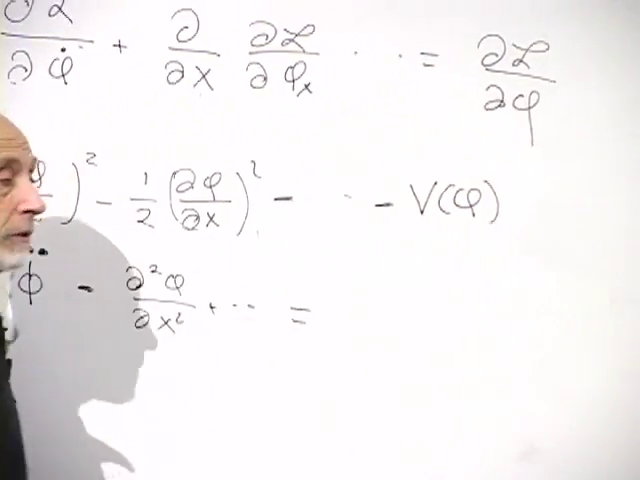
\includegraphics[width=0.74\textwidth]{lecture_09_figure_04.png}
\caption{尤拉--拉格朗日方程、標量場拉格朗日量，以及由\(V(\phi)\)所產生的場方程。}
\lectureframe{00:08:23}
\end{figure}

這就是標量場拉格朗日量所產生的方程。\editorialnote{保留的畫面左側遭到裁切；根據緊接著的口頭推導，可以確定此處顯示的補全內容。}

這裡\(V(\phi)\)是場的勢能密度。\(V\)中的常數項不影響這條方程，因為它的導數為零。線性勢在代數上雖然可行，卻沒有下界：場的能量可以一路降至負無窮。因此，第一個穩定的例子是
\begin{equation}
V(\phi)=\frac12m^2\phi^2,
\qquad
V'(\phi)=m^2\phi,
\end{equation}
它導出
\begin{equation}
\ddot\phi-\nabla^2\phi=-m^2\phi.
\end{equation}

為了看出\(m\)的物理意義，代入平面波
\begin{equation}
\phi(\mathbf x,t)=\phi_0e^{i\omega t-i\mathbf k\cdot\mathbf x}.
\end{equation}
於是
\begin{equation}
\ddot\phi=-\omega^2\phi,
\qquad
\nabla^2\phi=-\mathbf k^2\phi,
\end{equation}
波動方程便成為
\begin{equation}
-\omega^2\phi+\mathbf k^2\phi=-m^2\phi.
\end{equation}
消去\(\phi\)後，得到
\begin{equation}
\omega^2=\mathbf k^2+m^2.
\end{equation}
在\(\hbar=c=1\)單位制中，頻率對應能量，波數對應動量。因此
\begin{equation}
E^2=\mathbf p^2+m^2,
\end{equation}
或者，恢復\(c\)的冪次後，\(E^2=\mathbf p^2c^2+m^2c^4\)。參數\(m\)就是場的一個量子的質量。

可以直接在簡潔的表示式層次要求洛倫茲不變性。若\(\mathcal L\)是洛倫茲純量，它所導出的運動方程就是洛倫茲不變的。時間導數與空間導數之間的相對符號，正是狹義相對論中熟悉的時空符號差異。

\section{非線性與耦合的經典場}

場的高次項會帶來新的行為。若
\begin{equation}
V(\phi)=\frac12m^2\phi^2+g\phi^3,
\end{equation}
則
\begin{equation}
\ddot\phi-\nabla^2\phi=-m^2\phi-3g\phi^2.
\end{equation}
拉格朗日量中的二次項會導出場的線性方程；三次及更高次項則會導出非線性方程。

波包的運動清楚呈現了這項差異。對於線性方程，向右行進的波包與向左行進的波包可以相加，形成另一個解。兩者重疊並干涉一段時間，接著彼此穿越，離開時仍保持原有形狀。若有非線性項，波包便會彼此影響；它們可能散射、變形，或分裂成更複雜的波。線性波暫時干涉並不代表交互作用；波包持續改變，才是非線性的表徵。

兩個標量場也會呈現相同的模式。令
\begin{align}
\mathcal L
&=
\frac12(\partial_\mu\phi)(\partial^\mu\phi)
+\frac12(\partial_\mu\rho)(\partial^\mu\rho)
-V(\phi,\rho),
\\
V(\phi,\rho)
&=
\frac12m^2\phi^2+\frac12M^2\rho^2+\rho\phi^2.
\end{align}
若沒有最後一項，兩個方程彼此獨立：
\begin{equation}
\ddot\phi-\nabla^2\phi=-m^2\phi,
\qquad
\ddot\rho-\nabla^2\rho=-M^2\rho.
\end{equation}
它們描述兩種粒子的量子，質量分別為\(m\)與\(M\)。加入混合項後，
\begin{align}
\ddot\phi-\nabla^2\phi&=-m^2\phi-2\rho\phi,
\\
\ddot\rho-\nabla^2\rho&=-M^2\rho-\phi^2.
\end{align}
每個方程現在都包含另一個場。這些方程彼此耦合，而且是非線性的：一個\(\phi\)波包會散射一個\(\rho\)波包，反之亦然。導數項決定能量--動量關係；未微分的二次項決定質量；混合的高次項則描述交互作用。這就是基本的經典模式。

\section{狄拉克場與標量耦合}

狄拉克場的方程對時間是一階的。以下以一維簡寫，並假設可推廣至三個空間方向，其項的結構為
\begin{equation}
i\dot\Psi
\simeq
i\alpha\frac{\partial\Psi}{\partial x}+m\beta\Psi,
\qquad
i\boldsymbol\alpha\cdot\boldsymbol\nabla\Psi
=i\sum_i\alpha_i\frac{\partial\Psi}{\partial x_i}.
\end{equation}
矩陣\(\alpha_i\)與\(\beta\)作用於\(\Psi\)的各個分量。相應的拉格朗日量包含一個對\(\partial_t\Psi\)呈線性的項、一個涉及\(\alpha_i\)的空間導數雙線性項，以及質量雙線性項\(m\Psi^\dagger\beta\Psi\)。此處只需掌握這項結構事實。\editorialnote{原文嘗試寫出的狄拉克拉格朗日量中，正負號、括號及\(i\)的位置都明確未定，因此無法據此推定任何依賴慣例的精確公式。}

\begin{figure}[htbp]
\centering
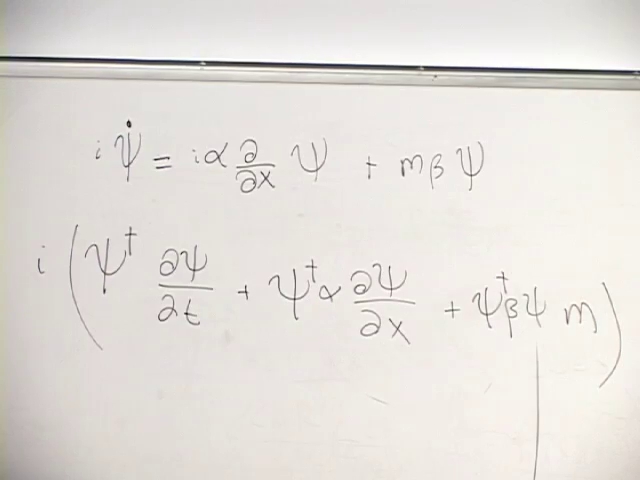
\includegraphics[width=0.76\textwidth]{lecture_09_figure_05.png}
\caption{狄拉克場討論中的時間導數項、空間導數項與質量項。}
\lectureframe{00:25:37}
\end{figure}

\begin{classroomqa}
\lecturetimestamp{00:26:37}
\audiencequestion{嘗試寫出的狄拉克拉格朗日量中，括號的位置是否正確？也就是說，\(i\)是否乘上整個表示式？}
\lecturerresponse{此處無法有把握地確定括號的位置，而且結構上的重點也不需要它：確實存在一個能導出狄拉克方程的拉格朗日量。}
\end{classroomqa}

現在加入標量場\(\phi\)。直接取乘積\(\Psi^\dagger\Psi\,\phi\)並不是洛倫茲純量。若插入質量項中出現的同一個狄拉克矩陣，就得到
\begin{equation}
\mathcal L_{\mathrm{int}}
\propto
\Psi^\dagger\beta\Psi\,\phi.
\end{equation}
換句話說，\(\Psi^\dagger\beta\Psi\)是標量狄拉克雙線性。對完整拉格朗日量作變分，會在狄拉克方程中加入一項，其正比於\(\phi\)；在標量方程中則加入一個正比於\(\Psi^\dagger\beta\Psi\)的源項。兩個場會彼此散射。

\begin{classroomqa}
\lecturetimestamp{00:28:03}
\audiencequestion{標量--費米子交互作用中插入的\(\beta\)，是否與狄拉克質量項中的\(\beta\)相同？}
\lecturerresponse{是，同一個狄拉克矩陣。}
\end{classroomqa}

比較
\begin{equation}
m\Psi^\dagger\beta\Psi
\qquad\hbox{and}\qquad
\Psi^\dagger\beta\Psi\,\phi
\end{equation}
可以看出，這種耦合的形式就像以標量場取代質量參數。接近本章末尾討論具有非零真空值的場時，還會再看到這個觀察。

到目前為止，這裡的詮釋都屬於經典描述：波包散射其他波包。場成為算符後，同一套代數便有了更明確的粒子意義。

\section{量子場的冪次所代表的過程}

實標量量子場同時包含產生算符與湮滅算符。示意地寫成
\begin{equation}
\phi(x)\sim A^+(x)+A^-(x),
\end{equation}
其中\(A^+\)產生一個量子，\(A^-\)湮滅一個量子。因此，\(\phi^3(x)\)包含四種局域過程：
\begin{equation}
\phi^3
\sim
(A^+)^3+(A^+)^2A^-+A^+(A^-)^2+(A^-)^3,
\end{equation}
以下的示意解讀省略了排序細節與數值係數。粒子數的四種變化分別是
\begin{equation}
3\longrightarrow0,
\qquad
0\longrightarrow3,
\qquad
2\longrightarrow1,
\qquad
1\longrightarrow2.
\end{equation}
三個場因子都作用在同一點\(x\)。因此，一個三次項就包含三個粒子湮滅、三個粒子產生、兩個量子合併成一個，以及一個量子分裂成兩個。在物理振幅中，能量--動量守恆之後可能排除其中一些局域解讀；但它們都存在於算符乘積本身。

二次自由項的作用則不同。先暫不考慮相鄰點\(x\)與\(x'\)之間差值的歸一化因子：
\begin{equation}
\partial_x\phi
\ \propto\
\phi(x)-\phi(x').
\end{equation}
將差值平方並展開，可得以下項的結構：
\begin{align}
\frac12(\partial_x\phi)^2
&\ \propto\
\frac12\bigl[\phi(x)-\phi(x')\bigr]^2
\\
&=
\frac12\phi(x)^2
+\frac12\phi(x')^2
-\phi(x)\phi(x').
\end{align}
每個同一點的平方項都有幾種算符解讀：可以在同一點產生兩個量子、湮滅兩個量子，或在該點湮滅一個量子後再將它產生。這些項不會使粒子從一處移動到另一處。交叉項則可以在\(x'\)湮滅一個量子，並在\(x\)產生該量子，反向過程也可以。因此它相當於最近鄰躍遷項。反覆作用的因子會將粒子從\(x\)帶至\(x'\)，再到\(x''\)，如此繼續。二次導數項支配自由傳播；三次及更高次項則使粒子散射、產生與湮滅。

\begin{classroomqa}
\lecturetimestamp{00:36:07}
\audiencequestion{導數的有限差分表示式是否應包含間隔\(x-x'\)？}
\lecturerresponse{是。將間隔記為\(L\)後，差值平方會帶出因子\(L^{-2}\)。這個數值因子會改變係數，但不影響躍遷的詮釋。}
\end{classroomqa}

恢復間隔後，得到
\begin{align}
\frac12(\partial_x\phi)^2
&\longrightarrow
\frac{1}{2L^2}\bigl[\phi(x)-\phi(x')\bigr]^2
\\
&=
\frac{1}{2L^2}\phi(x)^2
+\frac{1}{2L^2}\phi(x')^2
-\frac{1}{L^2}\phi(x)\phi(x').
\end{align}

質量項也是二次項，但不含導數：
\begin{equation}
\frac12m^2\phi(x)^2.
\end{equation}
就單粒子而言，可以將它解讀為入射量子在同一點被吸收後再重新發射。它不會使量子移動；它為量子在該處的存在賦予權重，或者說，在這個意義上計數。同一個算符平方也包含雙產生與雙湮滅的解讀。因此，就運動而言，關鍵差異在於連結相鄰點的交叉項，以及作用於單一點內的質量插入。

\section{量子電動力學的局域頂點}

這些基本粒子過程的示意圖，正是費曼圖的起點。核心例子是量子電動力學，也就是描述電子、正電子與光子的理論。

狄拉克方程具有正能量模與負能量模。依較早期的說法，\(\Psi\)包含兩類模式的湮滅算符，而\(\Psi^\dagger\)則包含相應的產生算符。移除一個負能量電子，可以重新詮釋為產生一個正能量正電子。重新標記後，方便的示意分解為
\begin{align}
\Psi
&\sim
C^-_{e^-}+C^+_{e^+},
\\
\Psi^\dagger
&\sim
C^+_{e^-}+C^-_{e^+}.
\end{align}
因此，\(\Psi\)會湮滅電子或產生正電子；\(\Psi^\dagger\)則會產生電子或湮滅正電子。這個簡寫不包含任何歸一化因子、自旋標記或動量積分。

QED交互作用將狄拉克流與電磁向量勢耦合。在此使用的分量記號中，其結構為
\begin{equation}
\mathcal L_{\mathrm{QED,int}}
\sim
e\left(
\Psi^\dagger\Psi\,A_0
+
\Psi^\dagger\boldsymbol{\alpha}\Psi\mathbin{\boldsymbol{\cdot}}\mathbf A
\right),
\end{equation}
其中
\begin{equation}
J^0=\Psi^\dagger\Psi,
\qquad
\mathbf J=\Psi^\dagger\boldsymbol{\alpha}\Psi.
\end{equation}
符號\(\sim\)很重要：時間項與空間項的相對符號取決於度規和向量勢的慣例。不依賴慣例的說法是，四維流與四維勢作縮並。\editorialnote{原文給出了流的時間與空間分量，但未確定分量縮並所採用的度規慣例。}

光子場 \(A_\mu\) 本身包含光子的產生算符和湮滅算符。它的向量性質還承載光子的極化---這個小小的方向性 ``標誌''，以及光子的動量。

\begin{classroomqa}
\lecturetimestamp{00:44:28}
\audiencequestion{當\(A_\mu\)是向量，而費米子因子乍看之下是純量時，交互作用怎麼會是純量？}
\lecturerresponse{費米子也提供四維向量：\(\Psi^\dagger\Psi\)是時間分量，\(\Psi^\dagger\boldsymbol\alpha\Psi\)是空間分量。將這個流與\(A_\mu\)縮並，就會得到純量。}
\end{classroomqa}

將\(\Psi^\dagger\)、\(\Psi\)和\(A_\mu\)的算符內容相乘，就會得到同一個局域頂點的四種常見解讀：
\begin{enumerate}
\item 電子發射光子；
\item 電子吸收光子；
\item 電子與正電子湮滅，產生光子；
\item 光子產生電子--正電子對。
\end{enumerate}
以第一種解讀為例，\(\Psi\)湮滅入射電子，\(\Psi^\dagger\)產生出射電子，而光子場則產生光子。若選用光子的湮滅部分，便得到吸收過程；若選用正電子部分，則得到正負電子對的湮滅或產生。一個局域項就包含了這一整組過程。

在費米子流圖中，正電子線上的箭頭方向與正電子的傳播方向相反。依照這項慣例，費米子流的箭頭會連續穿過每一個允許的QED頂點。四種解讀的差異在於外線移至入射側或出射側，而不是費米子流線中斷。

每一種解讀都帶有相同的係數\(e\)，也就是此處微觀慣例下的電荷。這個係數是電荷\(e\)，不是精細結構常數，儘管兩者密切相關。頂點振幅正比於\(e\)；納入所有運動學與歸一化因子後，相應的機率尺度正比於\(e^2\)。

\begin{classroomqa}
\lecturetimestamp{00:49:44}
\audiencequestion{將光子解讀為轉變成電子--正電子時，頂點係數是否與其他解讀相同？}
\lecturerresponse{是，電荷係數同樣是\(e\)。}
\end{classroomqa}

\begin{classroomqa}
\lecturetimestamp{00:49:59}
\audiencequestion{機率沒有單位，是否仍需要一個尺度因子？}
\lecturerresponse{在此採用的自然微觀慣例中，電荷\(e\)是無因次的。它決定振幅的尺度，而它的平方決定機率的尺度。}
\end{classroomqa}

可以想像電子撞上牆壁並突然停下。能量與動量有一定機率以光子的形式離開。輻射振幅中基本的電磁因子是\(e\)，因此機率尺度包含\(e^2\)。這裡指出的是耦合因子；實際機率也取決於電子的狀態與運動學。

\begin{figure}[htbp]
\centering
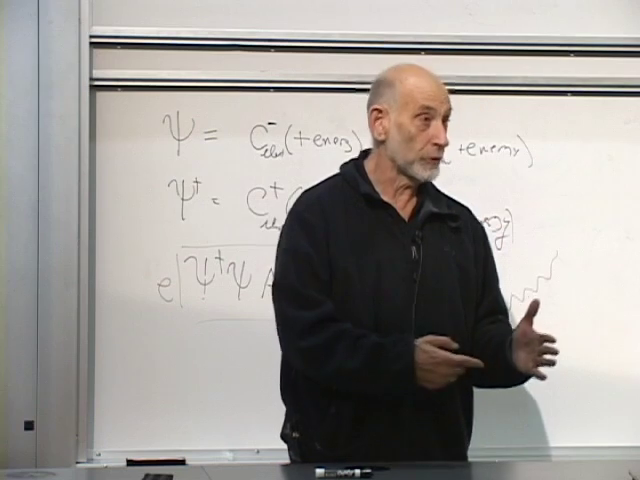
\includegraphics[width=0.78\textwidth]{lecture_09_figure_06.png}
\caption{\(\Psi\)與\(\Psi^\dagger\)所含的電子與正電子算符，以及電子--光子交互作用示意圖。}
\lectureframe{00:50:39}
\end{figure}

\begin{classroomqa}
\lecturetimestamp{00:51:15}
\audiencequestion{電荷有單位嗎？}
\lecturerresponse{在此使用的自然微觀慣例中，電荷沒有單位。宏觀電荷常以庫侖表示，但粒子理論以選定的基本單位為基準來衡量電荷。在普朗克單位或其他自然單位制中，這些量都以純數表示。}
\end{classroomqa}

這是慣例與尺度的差異。庫侖適合表示導線中的電流；無因次耦合則適合描述微觀振幅。\editorialnote{在00有個簡短提問：52：37--00：53：15關於如何``分組''含電荷的項，原文表述嚴重受損，因此無法確定其意圖。}

基本QED交互作用中的三個場，都在同一個時空點取值。頂點本身沒有內部時間延遲。

\begin{classroomqa}
\lecturetimestamp{00:53:19}
\audiencequestion{電子的吸收與再發射，以及光子的發射，是同時發生的嗎？還是方程中內含某種延遲？}
\lecturerresponse{在基本頂點處，所有算符都在同一個時空點取值。因此，這個基本過程中各項作用之間沒有延遲。}
\end{classroomqa}

\begin{classroomqa}
\lecturetimestamp{00:53:57}
\audiencequestion{每一種守恆量都必須各自守恆嗎？}
\lecturerresponse{是。電荷就是必須各自守恆的量之一。}
\end{classroomqa}

電荷守恆在圖像和代數中都看得出來。若入射電子變成出射正電子，電荷就會反轉，因此這不是允許的QED頂點。若時間軸朝上，電子箭頭朝上，正電子箭頭則朝下；合法的頂點總會有一條貫穿頂點的費米子箭頭。在代數上，交互作用包含一個\(\Psi\)和一個\(\Psi^\dagger\)。前者在湮滅電子或產生正電子時，會使電荷增加一個單位；後者則使電荷減少一個單位。兩者的效果相互抵消。

\begin{classroomqa}
\lecturetimestamp{00:56:05}
\audiencequestion{方框中的電子--光子表示式就是完整的QED拉格朗日量嗎？}
\lecturerresponse{不是。它是交互作用項。支配傳播的自由光子二次項與狄拉克二次項都尚未寫出。}
\end{classroomqa}

\begin{classroomqa}
\lecturetimestamp{00:56:35}
\audiencequestion{經典拉格朗日量是推導出來的，而量子拉格朗日量則是猜測後再加以檢驗的嗎？動能減去勢能的結構在量子力學中也保留嗎？}
\lecturerresponse{動能減去勢能的形式仍然保留：時間導數提供動能形式，空間梯度將這種形式推廣，而未微分的場項提供勢能形式。量子拉格朗日量是更基本的描述。在含有大量量子的狀態中，同一個拉格朗日量會導出經典波動方程。候選拉格朗日量依據物理原理與更深層的理論提出，再透過碰撞實驗加以確立或排除。}
\end{classroomqa}

大量子佔據的極限，說明了為何同一個表示式能支配量子粒子理論及其經典波。這種一致性並非事後另行強加的結果；經典場是大量量子的集體行為。反過來說，實驗碰撞能直接呈現基本頂點，讓人得以極精確地確定QED與標準模型中的交互作用。

\section{交叉與時空守恆定律}

局域頂點的外線可以在入射位置與出射位置之間互換。將一條出射粒子線移到入射側時，必須將它重新詮釋為相應的反粒子，反過來也一樣。從這個角度看，同一個電子--正電子--光子算符，可以有發射、吸收、正負電子對湮滅、正負電子對產生，甚至所有粒子皆從入射側進入的局域解讀。

\begin{classroomqa}
\lecturetimestamp{00:59:34}
\audiencequestion{將基本頂點圖旋轉後，它仍代表一種有效的局域解讀嗎？}
\lecturerresponse{是。外線可以在入射與出射位置之間移動，並相應地將粒子--重新詮釋為反粒子，或反之。}
\end{classroomqa}

局域算符的解讀還不是完整的物理過程。必須對頂點可能發生的所有時空點積分。時間積分使能量守恆，空間積分使動量守恆。電子、正電子與光子全都消失於真空的圖像，雖然是算符的一種形式上的局域解讀，但積分後的振幅為零，因為這個過程無法同時滿足能量與動量守恆。

\begin{classroomqa}
\lecturetimestamp{01:00:30}
\audiencequestion{所有粒子都從入射側進入的圖像，是否表示電子、正電子與光子可以消失得無影無蹤？}
\lecturerresponse{這是對局域算符的一種解讀，但物理振幅還包含對頂點位置的積分。這些積分會要求能量與動量守恆，因此這個運動學上不允許的過程，其振幅為零。}
\end{classroomqa}

\begin{classroomqa}
\lecturetimestamp{01:01:57}
\audiencequestion{反向的真空轉變成電子--正電子--光子這種解讀是否也存在？被排除的過程是否會在積分後消失？}
\lecturerresponse{反向的局域解讀同樣存在。對空間與時間積分後，任何不符合守恆定律的過程都會被排除。}
\end{classroomqa}

拉格朗日量中的導數可以套用到算符展開上，而不必對產生與湮滅符號本身微分。場的形式示意如下：
\begin{equation}
\Psi(x)
\sim
\int d^3k\,
\bigl[
C(\mathbf k)e^{i\mathbf k\cdot\mathbf x-i\omega t}
+\cdots
\bigr].
\end{equation}
算符\(C(\mathbf k)\)是時空展開中的係數。導數作用於平面波，會帶下\(\mathbf k\)或\(\omega\)。

\begin{classroomqa}
\lecturetimestamp{01:02:27}
\audiencequestion{對場展開式微分時，產生算符本身也要微分嗎？}
\lecturerresponse{不用。在這個展開式中，產生與湮滅算符不依賴時空座標。導數作用於指數因子，帶下動量與頻率。}
\end{classroomqa}

\section{核子與{\proseunicodefont π}介子：有效理論}

同樣的語言也能用來描述質子、中子與{\proseunicodefont π}介子。質子與中子是費米子，分別以場\(\Psi_p\)和\(\Psi_n\)表示。在這段討論交互作用計數的內容中，{\proseunicodefont π}介子場視為三種帶電狀態的純量場：
\begin{equation}
\pi^+,
\qquad
\pi^-,
\qquad
\pi^0.
\end{equation}
質子與\(\pi^+\)各帶一個正電荷單位；\(\pi^-\)帶一個負電荷單位；中子與\(\pi^0\)則不帶電。從更深層的觀點來看，{\proseunicodefont π}介子是夸克--反夸克組成的系統，但一開始可以先不處理其內部結構。

一組示意性的核子--{\proseunicodefont π}介子場乘積如下，並符合電荷守恆：
\begin{equation}
\mathcal L_{N\pi}
\sim
\left\{
\Psi_p^\dagger\Psi_n\,\pi^+,\;
\Psi_n^\dagger\Psi_p\,\pi^-,\;
\Psi_p^\dagger\Psi_p\,\pi^0,\;
\Psi_n^\dagger\Psi_n\,\pi^0
\right\}.
\end{equation}
這裡只列出場的內容與電荷配置；相對係數、正負號及旋量矩陣結構都尚未確定。第一個{\proseunicodefont π}介子場的電荷，可藉由檢驗一種具體解讀來判定：中子和正{\proseunicodefont π}介子可以產生質子；若在此處改用負{\proseunicodefont π}介子，便會使負的入射電荷轉變為正的出射電荷。共軛項則描述反向的帶電過程。\editorialnote{原文多次修正{\proseunicodefont π}介子的電荷符號，最後才得到此處所示、符合電荷守恆的一對項；目前的排列呈現其最後採用的示意結構。}

每一項同樣有數種交叉解讀。將出射中子移到入射側時，它就改以入射反中子的身分出現。因此，帶電頂點可以描述質子與反中子結合成\(\pi^+\)，也可以描述運動學條件允許時的\(p\to n+\pi^+\)等過程。中性項則允許質子或中子發射或吸收\(\pi^0\)。電荷守恆決定哪些過程屬於允許的範圍；能量、動量及其他可能的對稱性，則決定特定實驗中實際可能發生哪一種過程。

在夸克的內部結構尚未為人所知時，這是一種實用的有效描述。只要探測無法分辨內部結構，它就仍然有用。質子的組成成分分布在有限的範圍內，有些像具有內部結構的原子，只是尺度小得多。如果實驗中的動量轉移太小，無法打散或解析質子，就可以把質子視為具有自身場的點粒子。碰撞能量足夠高時，夸克便會顯現，這時點粒子質子場就不再足以描述系統。

質子帶電，因此也有局域的質子--光子交互作用，示意寫成\(J_p^\mu A_\mu\)，其中\(J_p^\mu\)是質子流。電子也有相應的電子--光子交互作用。質子不能藉由發射光子而轉變成中子：\(p\to n+\gamma\)不符合電荷守恆。

\begin{classroomqa}
\lecturetimestamp{01:10:28}
\audiencequestion{質子與電子交互作用時會發生什麼？}
\lecturerresponse{帶電粒子各自都有光子頂點。質子可以發射光子而仍保持為質子；電子則可以吸收光子而仍保持為電子。質子--電子散射由這兩個局域頂點，以及光子在兩者之間的傳播組合而成。}
\end{classroomqa}

\section{局域性與基本過程的反覆作用}

描述完整的質子--電子交換，並不需要特殊的非局域項。一個局域頂點使光子在質子處產生；光子的二次項將它從一個鄰近點傳到另一個鄰近點；接著，另一個局域頂點使電子吸收光子。這個延展的過程由這些基本部分組合而成。
\begin{equation}
\begin{aligned}
\bigl[J_p^\mu A_\mu\bigr](x_p)
&\longrightarrow
\underbrace{x_p\to x_1\to x_2\to\cdots\to x_e}_{\text{quadratic photon propagation}}
\\
&\longrightarrow
\bigl[J_e^\nu A_\nu\bigr](x_e).
\end{aligned}
\end{equation}
這條示意鏈上的箭頭表示依序在相鄰點插入，而不是表示一種新的非局域交互作用。

\begin{classroomqa}
\lecturetimestamp{01:12:06}
\audiencequestion{整個質子--電子交換過程的拉格朗日量該如何寫？}
\lecturerresponse{不會為整個延展過程另加一項。這個過程由局域的質子--光子頂點、重複出現的二次傳播項，以及局域的電子--光子頂點構成。}
\end{classroomqa}

局域結構有兩種形式。未含導數的相互作用項作用於單一時空點。以有限差分表示的導數項，則只連結該點與鄰近點。這兩種形式都不會讓粒子直接跨越有限距離。長程傳播是由許多無窮小的步驟組成；不存在基本的超距作用。

\begin{classroomqa}
\lecturetimestamp{01:14:36}
\audiencequestion{拉格朗日量中的項都只作用於單一點嗎？}
\lecturerresponse{相互作用項作用於單一點。導數項連結一個點與無窮接近的鄰點。發射、許多次相鄰跳躍以及吸收，共同形成有限距離的交換。}
\end{classroomqa}

\begin{classroomqa}
\lecturetimestamp{01:15:36}
\audiencequestion{延展過程中的所有部分都包含在內嗎？把它們組合起來，是否就是相乘？}
\lecturerresponse{是的。每一次基本的發射、跳躍或吸收都編碼在拉格朗日量中。反覆插入各項所形成的乘積，會將這些部分組合成較大的過程。}
\end{classroomqa}

這裡討論的相對論量子場論，預設了場所定義於其中的時空背景。不應將它與描述動態時空幾何的完整量子理論混為一談。

\begin{classroomqa}
\lecturetimestamp{01:16:28}
\audiencequestion{在黑洞視界附近等強烈相對論情況下，這種組合方式仍然成立嗎？}
\lecturerresponse{將這套構造延伸至黑洞問題，超出了此處討論的範圍。這裡採用的量子場論本身，無法完整描述黑洞動力學；在那種情況下，引力不可或缺。}
\end{classroomqa}

場是描述基本局域作用的算符。一個場因子可以吸收一個粒子，也可以發射一個粒子。兩個因子的乘積可以在同一點吸收一個粒子並發射另一個粒子；更高次的乘積則能進一步改變粒子組成。局域算符的乘積將這些作用串接成一段歷程。在時空中，運動可表示為：粒子在一個小區域被吸收，再發射至鄰近區域，接著再次被吸收並再次發射。當步長趨近於零、步數不斷增加時，就得到連續軌跡。

\begin{classroomqa}
\lecturetimestamp{01:17:30}
\audiencequestion{在這種局域步驟的圖像中，該如何理解場、距離和時間？}
\lecturerresponse{場是描述局域吸收與發射的算符。這些基本作用透過乘積串接起來；穿越時空的運動則由無窮小的相鄰步驟構成，最後再取連續極限。}
\end{classroomqa}

因此，可以先將時空劃分成小單元，並將場算符配置在各個單元上，作為調節後的起點。\editorialnote{在01至17:30--01至20:40這段，聽眾的提問有部分聽不清楚；轉述只保留了仍可辨認的主題，而關於局域算符和連續時空步驟的回答則很清楚。}導數變成差分。二次交叉項連結相鄰單元，質量項和相互作用項則作用於單一單元內。這些單元是用來定義極限理論的工具，不是額外的粒子，也不代表新的物理質量尺度。

不必在每一步另外加入狹義相對論效應。當拉格朗日量是洛侖茲純量時，由它組成的振幅便具有洛侖茲不變性；時間膨脹等效應已由這種結構推導而出。

\begin{classroomqa}
\lecturetimestamp{01:21:10}
\audiencequestion{多步過程中的高速運動和時間膨脹會帶來額外問題嗎？}
\lecturerresponse{不需要另外修正。如果拉格朗日量是洛侖茲純量，時間膨脹等狹義相對論效應就已包含在結果之中。至於提問者確切關切的是什麼，則不完全清楚。}
\end{classroomqa}

產生算符和湮滅算符可以用位置表象或動量表象表示。位置空間中的產生算符，是動量空間中產生算符的傅立葉疊加，反之亦然。不存在能產生位置和動量都精確確定之態的算符。要使粒子的位置高度局域化，就需要涵蓋很廣動量範圍；若使粒子的動量高度局域化，它的位置就會分散開來。用這套語言來說，兩種表象之間的傅立葉關係就是不確定性原理。

\begin{classroomqa}
\lecturetimestamp{01:22:48}
\audiencequestion{產生算符和湮滅算符與位置、動量及不確定性原理有什麼關係？}
\lecturerresponse{它們可以表示為位置的函數，也可以表示為動量的函數；兩種表示互為傅立葉變換。位置高度局域化的態需要涵蓋許多不同動量，而動量高度局域化的態則會在位置上分散開來；不存在能同時產生位置\(x\)和動量\(p\)都精確確定之態的產生算符。}
\end{classroomqa}

現在可以完整說明元胞構造。以\(n\)標記元胞，並將導數替換成有限差分，例如
\begin{equation}
\partial_\mu\phi(x)
\longrightarrow
\frac{\phi_{n+\hat\mu}-\phi_n}{a},
\end{equation}
再將每一種場都放入每個元胞。一個二次交叉項會從一個元胞移除一個量子，並在相鄰元胞產生一個量子。調節後的表示式定義完成後，令間距\(a\)趨近於零，就得到連續理論。
\begin{equation}
\underbrace{\phi_n\phi_{n+\hat\mu}}_{\text{hop }n\leftrightarrow n+\hat\mu},
\qquad
\underbrace{m^2\phi_n^2}_{\text{same-cell mass insertion}}.
\end{equation}

\begin{classroomqa}
\lecturetimestamp{01:25:16}
\audiencequestion{可以完成將時空劃分為元胞的構造嗎？}
\lecturerresponse{可以。場以元胞為索引，導數改寫成有限差分，二次項則讓粒子在相鄰元胞之間跳躍。元胞大小趨近於零時，就恢復連續理論。}
\end{classroomqa}

電子透過二次項在元胞間跳躍，光子也一樣。電子和光子在同一元胞相遇時，量子電動力學（QED）的相互作用可以吸收並重新發射電子，同時產生或湮滅光子。標量場的質量項可解讀為發生在同一元胞內的過程：粒子進入該元胞又離開，其係數正比於\(m^2\)。這項不會造成跳躍。

\begin{classroomqa}
\lecturetimestamp{01:28:18}
\audiencequestion{元胞大小和質量係數有關嗎？}
\lecturerresponse{沒有關係。元胞大小是最終會取至零的調節間距；質量係數則是拉格朗日量中的獨立參數。}
\end{classroomqa}

\begin{classroomqa}
\lecturetimestamp{01:28:43}
\audiencequestion{將局域因子相乘，是在整個時空上構造聯合振幅，而不只是依時間排列成序列嗎？}
\lecturerresponse{是的。元胞涵蓋整個時空，各元胞的局域貢獻會在整個時空網格上組合起來。這個乘積為所需的局域事件和傳播步驟提供聯合振幅。}
\end{classroomqa}

\section{源、探測器及其間的動力學}

完整的過程是一段發生於時空中的歷程。初始條件由實驗者準備的狀態決定，末態條件則由探測器記錄的結果決定。熱燈絲發射電子就是一個簡單的源。在燈絲處，場算符產生入射電子；在探測器的位置，場算符則描述電子最終被吸收。

\begin{classroomqa}
\lecturetimestamp{01:29:30}
\audiencequestion{這種時空過程的起始階段是什麼？}
\lecturerresponse{過程是在源處準備的。熱燈絲發射電子就是一個簡單例子：燈絲處的場算符產生電子，而探測器處的場算符則指定最終的吸收事件。}
\end{classroomqa}

同一套構造也可以從真空出發來描述。源處的產生算符作用於真空，構成入射態；與探測器相關的湮滅算符則選出出射態。這些算符指定邊界條件，並不取代源與探測器之間整個區域的動力學。

\begin{classroomqa}
\lecturetimestamp{01:31:11}
\audiencequestion{若只在發射源處放入動力學，而不讓它遍及整個系統，這樣做會錯嗎？}
\lecturerresponse{會。從真空出發，用源算符準備入射粒子，再用探測器算符選出末態粒子。在兩者之間，拉格朗日量反覆插入並作用於整個時空，使粒子移動、產生或湮滅。}
\end{classroomqa}

插入足夠多次後，數個粒子便能同時穿越許多相鄰元胞；途中也可能有粒子被產生或湮滅。初始算符說明哪些粒子進入，末端算符說明探測器記錄到哪些粒子，而反覆作用的拉格朗日量則描述兩者之間的一切。

\begin{classroomqa}
\lecturetimestamp{01:33:24}
\audiencequestion{如果拉格朗日量可以任意多次插入，那麼是否要對插入位置積分？}
\lecturerresponse{是的。要對插入位置的時空座標積分。這裡不推導精確的費曼規則；目前的重點是，簡單的局域場表示式編碼了基本相互作用，而完整過程是由這些相互作用組成的。}
\end{classroomqa}

\section{相位對稱性、電荷與振幅}

將基本過程寫入拉格朗日量，也會讓其中的對稱性顯現出來。考慮電子場的整體相位變換，
\begin{equation}
\Psi\longrightarrow e^{i\theta}\Psi,
\qquad
\Psi^\dagger\longrightarrow e^{-i\theta}\Psi^\dagger,
\qquad
A_\mu\longrightarrow A_\mu.
\end{equation}
含有相同數量\(\Psi\)和\(\Psi^\dagger\)的項保持不變，因為相位彼此抵消。若兩者數量不同，該項就會多出一個相位因子。兩者數量相等，正是電荷守恆的代數表述。

這是拉格朗日量描述的一項核心優勢。場因子呈現基本過程，這些因子的組合呈現對稱性，而對稱性則呈現守恆定律。反覆插入使準備好的初態演化為所選定的末態，所得結果就是量子振幅。精確計算需要費曼規則，但其結構已清楚可見：局域作用會依守恆定律所允許的各種階數反覆出現。

\section{場的測量與對易子}

場算符仍具有量子力學中算符的一般意義。其本徵值是場測量可能得到的結果，本徵向量則描述與這些值相應的態。要探測電場，可以將帶電粒子置於其中，觀察粒子如何加速。

\begin{classroomqa}
\lecturetimestamp{01:37:06}
\audiencequestion{場算符的本徵值和本徵向量，是否仍發揮一般量子力學中的作用？}
\lecturerresponse{是。本徵值是可能測得的場值；場也可以透過其對粒子的作用來探測。對易子決定哪些量不能同時測量。}
\end{classroomqa}

平凡的恆等式
\begin{equation}
[\phi(x),\phi(x)]=0
\end{equation}
並未解決測量問題。必須先指定兩個可觀測量及其時空關係。場與其共軛動量構成一對正則的非對易量；在類時分離的點上，場算符不一定對易。相對地，類空分離的局域玻色場確實對易，這是局域性所要求的。因此，對易子與不確定性之間的熟悉關聯仍然適用，但必須先正確辨認所涉及的算符對。\editorialnote{原文對不同點的非對易性說得過於籠統。這裡的限定保留了其測量方面的重點，同時符合類空分離的局域玻色場必須滿足的微觀因果性。}

\begin{classroomqa}
\lecturetimestamp{01:39:57}
\audiencequestion{電場或電磁場的單位是伏特，還是伏特每公尺？}
\lecturerresponse{電場的單位是伏特每公尺。描述微觀場過程時，伏特和公尺不是最有用的語言；這類過程用光子來描述更自然。反過來說，量子場論也不是用來決定如何替房子澆水的合適語言。}
\end{classroomqa}

一種描述所適用的單位，不一定能讓另一種描述更清楚。伏特和伏特每公尺適用於宏觀儀器；光子的產生和湮滅則適用於微觀過程。

\begin{classroomqa}
\lecturetimestamp{01:41:10}
\audiencequestion{核心概念是否在於：拉格朗日量中的各項是組成較大過程的基本單元？}
\lecturerresponse{是。基本過程會從一個點延伸至相鄰的點，反覆發生。每個基本單元都作用於單一時空點，或透過導數項連結相鄰點。表面上非局域的傳播，是由這些局域步驟組成的；不存在基本的超距作用。}
\end{classroomqa}

\section{局域過程的乘積與路徑求和}

可以用一種簡潔的啟發式方式，呈現局域過程如何反覆出現。將時空劃分為元胞，並寫成
\begin{equation}
\prod_x\bigl(1+\mathcal L_I(x)\bigr),
\end{equation}
其中\(x\)標記元胞，\(\mathcal L_I(x)\)是局域相互作用拉格朗日量。這不是精確的連續時空公式，而是一種組合式的替代表示，用來呈現乘積如何生成局域事件所有可能的允許組合。

\begin{classroomqa}
\lecturetimestamp{01:42:18}
\audiencequestion{能否用一個式子簡潔表示多次產生、傳播和湮滅？}
\lecturerresponse{啟發式地說，對每個時空元胞都乘上一個因子\(1+\mathcal L_I(x)\)。展開乘積後，會得到沒有事件、在任一選定點發生一個事件，或在數個點發生事件等情形。}
\end{classroomqa}

對兩個元胞而言，
\begin{align}
\bigl(1+\mathcal L_I(x)\bigr)
\bigl(1+\mathcal L_I(x')\bigr)
&=
1+\mathcal L_I(x)+\mathcal L_I(x')
\notag\\
&\quad{}+\mathcal L_I(x)\mathcal L_I(x').
\end{align}
第一項表示兩處都沒有相互作用。接下來兩項則分別表示在\(x\)或\(x'\)發生一個基本相互作用。最後一項表示兩處都發生相互作用。因子多時，便會有涉及一個點、兩個點、三個點等等的項。含有多個頂點的項，例如可以描述兩個入射粒子產生三個出射粒子。

二次傳播項也納入同一套構造。有限位移可以表示為一串相鄰插入。在展開後的乘積中，會有一些因子分別位於某個元胞、它的鄰元胞、再下一個鄰元胞，依此類推，將粒子從一端帶到另一端。

\begin{classroomqa}
\lecturetimestamp{01:46:29}
\audiencequestion{有限距離的傳播需要許多局域運動項，那麼該如何得到所需的運動？}
\lecturerresponse{大型乘積中包含一串相鄰插入，可將粒子從初始點帶到終點。通常存在許多沿不同路徑連接兩點的序列。每條路徑都貢獻一個振幅，總振幅則是所有振幅的總和。}
\end{classroomqa}

若以\(r\)表示一條路徑，則示意地有
\begin{equation}
\mathcal A_{\mathrm{total}}=\sum_r\mathcal A_r,
\qquad
P=\left|\mathcal A_{\mathrm{total}}\right|^2.
\end{equation}
路徑的普通機率不是各自算出後再相加；而是先將振幅相加：
\begin{equation}
\left|\sum_r\mathcal A_r\right|^2
=
\sum_r|\mathcal A_r|^2
+
\sum_{r\ne s}\mathcal A_r\mathcal A_s^*.
\end{equation}
交叉項就是干涉項。

\begin{classroomqa}
\lecturetimestamp{01:48:27}
\audiencequestion{這與雙縫實驗的結果一致嗎？}
\lecturerresponse{完全一致。粒子通過兩條狹縫的兩種可能路徑，各自貢獻一個振幅。將振幅相加後再取平方，就會產生干涉項；局域步驟構造中的許多時空路徑也以相同方式相互干涉。}
\end{classroomqa}

\begin{classroomqa}
\lecturetimestamp{01:49:00}
\audiencequestion{\(1\)在每個因子\(1+\mathcal L_I\)中有什麼作用？}
\lecturerresponse{這是組合上的設計，讓每個元胞除了能貢獻一個相互作用，也能貢獻「沒有相互作用」的情形。它與路徑積分方法有關，但這裡寫出的乘積只是對技術性公式的啟發式近似。}
\end{classroomqa}

精確的形式體系會提供適當的時空積分、排序、歸一化和相位。這個乘積之所以有用，是因為它呈現了各種組合，卻不冒充完整的形式體系。

\begin{classroomqa}
\lecturetimestamp{01:49:57}
\audiencequestion{這就是作用量駐值原理嗎？}
\lecturerresponse{不是。經典駐值作用量原理會選出一條特定的經典軌跡；量子力學則是對各條軌跡的振幅求和，權重由作用量決定。即使某條路徑極其迂迴---例如從辦公室出發，先繞道巴黎，再前往附近的住家---也包含在量子求和之中。}
\end{classroomqa}

兩者的差別很簡單，儘管它們之間的關係細緻。在經典力學中，選出一條駐值路徑；量子力學則對所有路徑求和。在適當的極限下，經典軌跡附近的相位會彼此增強。

\section{推斷拉格朗日量與選擇作用範疇}

一旦給定拉格朗日量和指定的過程，計算其機率的規則就是確定的。計算仍可能需要巧思，正如解決艱深的數學問題往往需要巧思；但更深層的不確定性，在於找出自然界實際採用哪些場和耦合。

\begin{classroomqa}
\lecturetimestamp{01:50:43}
\audiencequestion{關鍵在於寫出拉格朗日量，還是在於使用它？}
\lecturerresponse{關鍵主要在於從實驗資料推斷拉格朗日量。一旦知道拉格朗日量，像是兩個粒子入射、四個粒子出射這樣的過程，就有確定的振幅，可依照明確規則計算。實際進行數學計算可能需要巧思，但這不是理論本身的不確定性。}
\end{classroomqa}

粒子碰撞能揭示基本頂點。人們提出各種項，通常以對稱性和更深層的原理為指引，再將計算所得的振幅與觀測結果比對。若結果吻合，就能確定哪些場的組合是允許的，以及相應的數值係數。

\begin{classroomqa}
\lecturetimestamp{01:52:24}
\audiencequestion{每種相互作用是否都有各自的拉格朗日量---還是有一本收錄許多拉格朗日量的大書？}
\lecturerresponse{目前採用的圖像則是：一個大拉格朗日量包含所有的場與相互作用，不過這個圖像最終可能不成立。可辨認的各個部分，都是這個總和中的組成部分。新粒子會增加一個場；新的基本過程則會增加一個相互作用項。}
\end{classroomqa}

完整的表示式可能雜亂，但不必長到足以編成一本書。粗略估計，可以假設有約一百種稱為基本粒子的對象，以及數百個項。量子電動力學、強作用、弱作用和引力範疇加在一起，仍可能只佔幾頁密密麻麻的文字。確切數目並不重要。實際採用的圖像是一個由許多可辨認部分組成的動力學表示式；而且明確來說，這個圖像最終可能會被證明並不完整。

這些場是否決定了更基本的時空幾何，已超出此處採用的標準量子場論架構所能處理的範圍。\editorialnote{關於01:55:00--01:55:20的提問損毀嚴重，無法可靠辨認它指的是哪個流形或幾何構造；只有這個界定討論範圍的回答可以確定。}

\begin{classroomqa}
\lecturetimestamp{01:55:22}
\audiencequestion{由實驗決定的數值就是耦合常數嗎？}
\lecturerresponse{耦合常數是拉格朗日量各項的係數。二次質量項的係數\(m^2\)就是一個例子；\(\phi^4\)、\(\phi^6\)或更高次冪項的係數也都是例子。}
\end{classroomqa}

同一個係數會控制一系列相關振幅，因為每個場乘積都可以有好幾種產生和湮滅的解讀。因此，知道拉格朗日量，就能決定遠不只一種孤立的反應。

\begin{classroomqa}
\lecturetimestamp{01:56:05}
\audiencequestion{要計算量子電動力學，是否必須知道完整的拉格朗日量？}
\lecturerresponse{若要達到無限精度，就必須知道所有能讓電子與光子相互作用的作用範疇。不過在原子能量範圍內，通常可以只考慮電子--光子作用範疇。能量不足以分辨細微的夸克結構，因此在所需的精度下，可以忽略其他作用範疇。}
\end{classroomqa}

實際計算會採用與實驗能量尺度相關的作用範疇。這就像流體力學：複雜的微觀系統可以用精確的粗粒化描述來處理，不必呈現所有更深層的組成。因此，量子場論可以同時具有唯象性和精確性---其採用的場與係數是唯象的，依據實驗推得；指定這些要素後所使用的規則則是精確的。

\begin{classroomqa}
\lecturetimestamp{01:58:09}
\audiencequestion{標準模型包含引力嗎？這些相對論性拉格朗日量包含廣義相對論嗎？}
\lecturerresponse{正式稱為標準模型的理論不包含引力，但討論更廣泛的理論時，可以把引力納入。這裡討論的場論結合了量子力學與狹義相對論，但本身並不包含廣義相對論。}
\end{classroomqa}

\section{真空值作為質量係數}

標量場的質量出現在\(\phi^2\)項的係數中。因此，若另一個場具有非零的真空值，它與標量場的交互作用就能呈現出質量項的效果。

\begin{classroomqa}
\lecturetimestamp{01:59:16}
\audiencequestion{如果粒子質量來自希格斯相互作用，那麼希格斯耦合能否起到質量項的作用？}
\lecturerresponse{可以。項\(H\phi^2\)是三次項，通常表示兩條\(\phi\)腿和一條\(H\)腿之間的相互作用。如果勢能\(V(H)\)選出\(H\)非零的真空值，該真空值便是一個乘在\(\phi^2\)上的數，因此會貢獻一個有效的二次質量項。}
\end{classroomqa}

示意地考慮
\begin{equation}
\mathcal L\supset H\phi^2-V(H).
\end{equation}
作為算符項，\(H\phi^2\)可以吸收一個\(\phi\)、發射一個\(\phi\)，並發射或吸收一個\(H\)量子。假設勢能在\(H=0\)以外有兩個極小值，而真空選擇其中一個：
\begin{equation}
\langle H\rangle=v\ne0.
\end{equation}
將場寫成真空值加上漲落，
\begin{equation}
H=v+h.
\end{equation}
於是
\begin{equation}
H\phi^2=v\phi^2+h\phi^2.
\end{equation}
第一項對\(\phi\)是二次的，會對其質量係數有所貢獻；第二項仍是與漲落場\(h\)之間的相互作用。\editorialnote{原文在說明非零真空值成為質量係數時便中斷了。此處展示的代換是直接的代數補全；正規化和正負號則取決於完整的拉格朗日量慣例。}

\begin{classroomqa}
\lecturetimestamp{02:01:29}
\audiencequestion{標準模型包含虛粒子的產生和湮滅嗎？}
\lecturerresponse{當然包含。虛粒子的產生和湮滅，是標準模型拉格朗日量所編碼的反覆量子過程中不可或缺的一部分。}
\end{classroomqa}
